\begin{frame}
\frametitle{About This Work...}

\emph{Managing Evolving Uncertainty in Trajectory Databases}~\cite{jeung2014managing}\\
H.~Jeung, H.~Lu, T.B.~Pedersen, S.~Sathe, M L.~Yiu.\\~\\

\begin{itemize}
  \item Published at \emph{TKDE' 2014}.
  \item A flexible trajectory modeling approach were proposed that takes into account model-inferred actual positions, time-varying uncertainty, and nondeterministic uncertainty ranges.
  \item Three estimators that effectively infer evolving densities of trajectory data were developed.
\end{itemize}

\end{frame}

%------------------------------------------------

\begin{frame}
\frametitle{Motivation}

\begin{itemize}
  \item \emph{Uncertainty management} is a central issue in trajectory databases
  \begin{fitemize}
    \item a common principle -- ``location uncertainty is captured by a certain range centered on the position recorded in the database''
  \end{fitemize}
  \item The old principle as the basis for the uncertain trajectory modelings is incapable of effectively capturing various types of uncertainty caused from different positioning sources
  \begin{fitemize}
    \item A location reported from a positioning system already bears some positional error, which implies that the exact location may not be identical to the reported position
    \item Positional errors may vary over time, as a result, the uncertainty should also change along time
    \item Bounding an area of uncertainty may cause loss of information
  \end{fitemize}
\end{itemize}

\end{frame}

%------------------------------------------------

\begin{frame}
\frametitle{Contributions}

\begin{itemize}

  \item \textbf{Evolving-density trajectory model}\quad to introduce a new uncertain trajectory model that represents a trajectory as time-dependent Gaussian distribution.

  \item \textbf{Evolving density estimators}\quad to propose three \emph{evolving density estimators} that infer time-varying densities of location data.

  \item \textbf{Efficient query processing}\quad to present an effective mechanism that indexes evolving density trajectories, and efficiently evaluates probabilistic range queries using the indexes.

\end{itemize}

\end{frame}

%------------------------------------------------

\begin{frame}
\frametitle{Existing Uncetain Trajectory Models}

There are two major reasons why uncertainty occurs in trajectory data:~\cite{pfoser1999capturing}
\begin{fitemize}
  \item one is known as \emph{measurement error} which is caused by limited accuracy of positioning technology, e.g., GPS error.
  \item the other is \emph{sampling error} that originates from discrete sampling of continuous movements of an object.
\end{fitemize}

Various \conceptbf{uncertainty models} have been proposed. These models commonly represent a trajectory using a sequence of uncertainty areas, so-called \emph{uncertain trajectory}.\\~\\

Each of the uncertainty areas captures the measurement and sampling errors.

\end{frame}

%------------------------------------------------

\begin{frame}
\frametitle{Existing Uncetain Trajectory Models}

\begin{figure}[tb]
  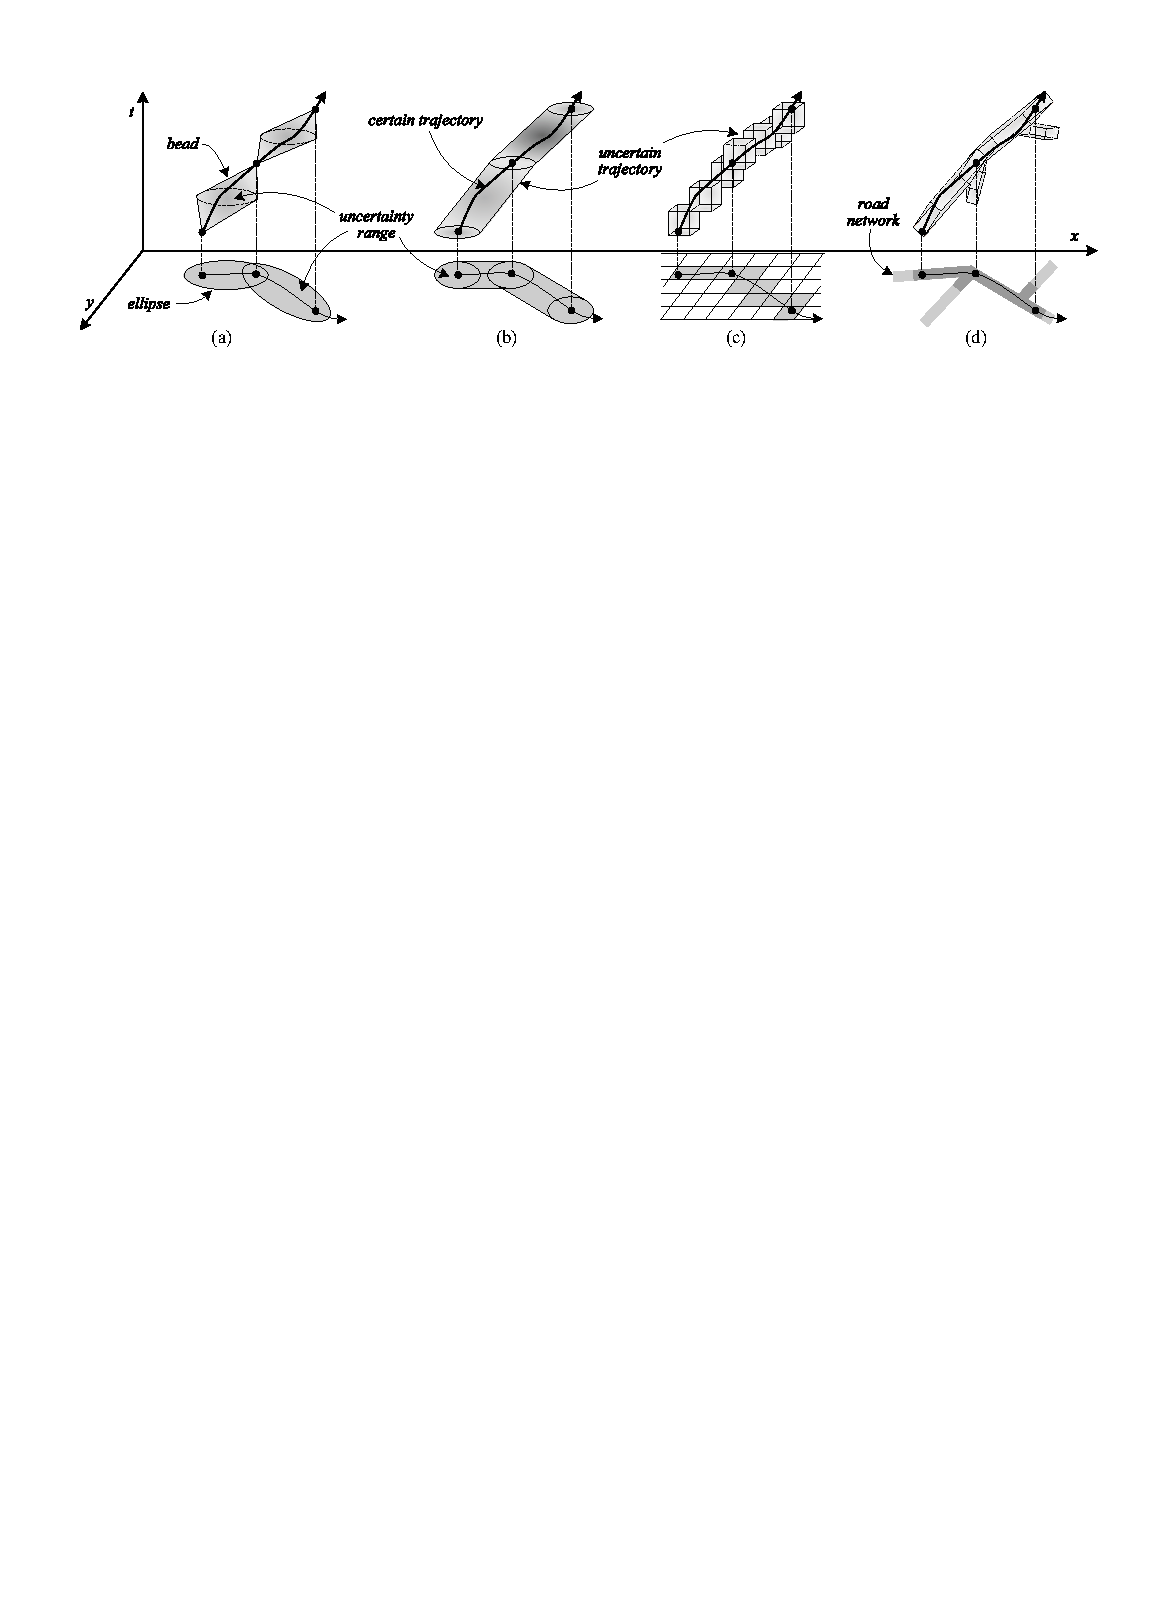
\includegraphics[width=\columnwidth]{figures/5-1/5-1-1.pdf}
\end{figure}

\vspace{10pt}

\footnotesize
\begin{tabular}{|l|c|c|c|c|}
\hline
\textbf{Models} & (a)Beads & (b)Cylinder & (c)Grid & (d)Network-constrained\\
\hline
\textbf{Works} & \cite{hornsby2002modeling,kuijpers2007trajectory} & \cite{frentzos2009effect,trajcevski2004managing,trajcevski2002geometry} & \cite{pelekis2009clustering,zhang2009effectively} & \cite{ding2008utr,ding2004uncertainty}\\
\hline
\end{tabular}

\end{frame}

%------------------------------------------------

\begin{frame}
\frametitle{Pitfalls of Existing Uncetain Trajectory Models}

\textrm{I.} \quad the uncertain trajectory models generally regard a location measured from positioning technology as a precise, actual location of an object, while modeling an uncertainty range based on the reported position as center.\\~\\

\textrm{II.} \quad some of the uncertain trajectory models assume that the degree of uncertainty is constant regardless of the cange of location or time.\\~\\

\textrm{III.} \quad the uncertain trajectory models bound the area of location uncertainty, typically using a circle with a user-specified radius. (\textit{it is inevitable to miss out some information when data processing is performed over any bounded uncertainty areas on unbounded distributions})

\end{frame}

%------------------------------------------------

\begin{frame}
\frametitle{Pitfalls of Existing Uncetain Trajectory Models}

\textrm{IV.} \quad most of the models assume that the probability density function (PDF) of a location is given, it is however a non-trival problem to compute the parameters of a PDF. \\~\\

\textrm{V.} \quad some models require additional data beyond location coordinates: the beads model uses maximum speed of object to determine the thickness of ellipse, while the network-constrained model needs map data encompassing the coverage of trajectories.

\end{frame}
